% !TEX encoding = UTF-8 Unicode
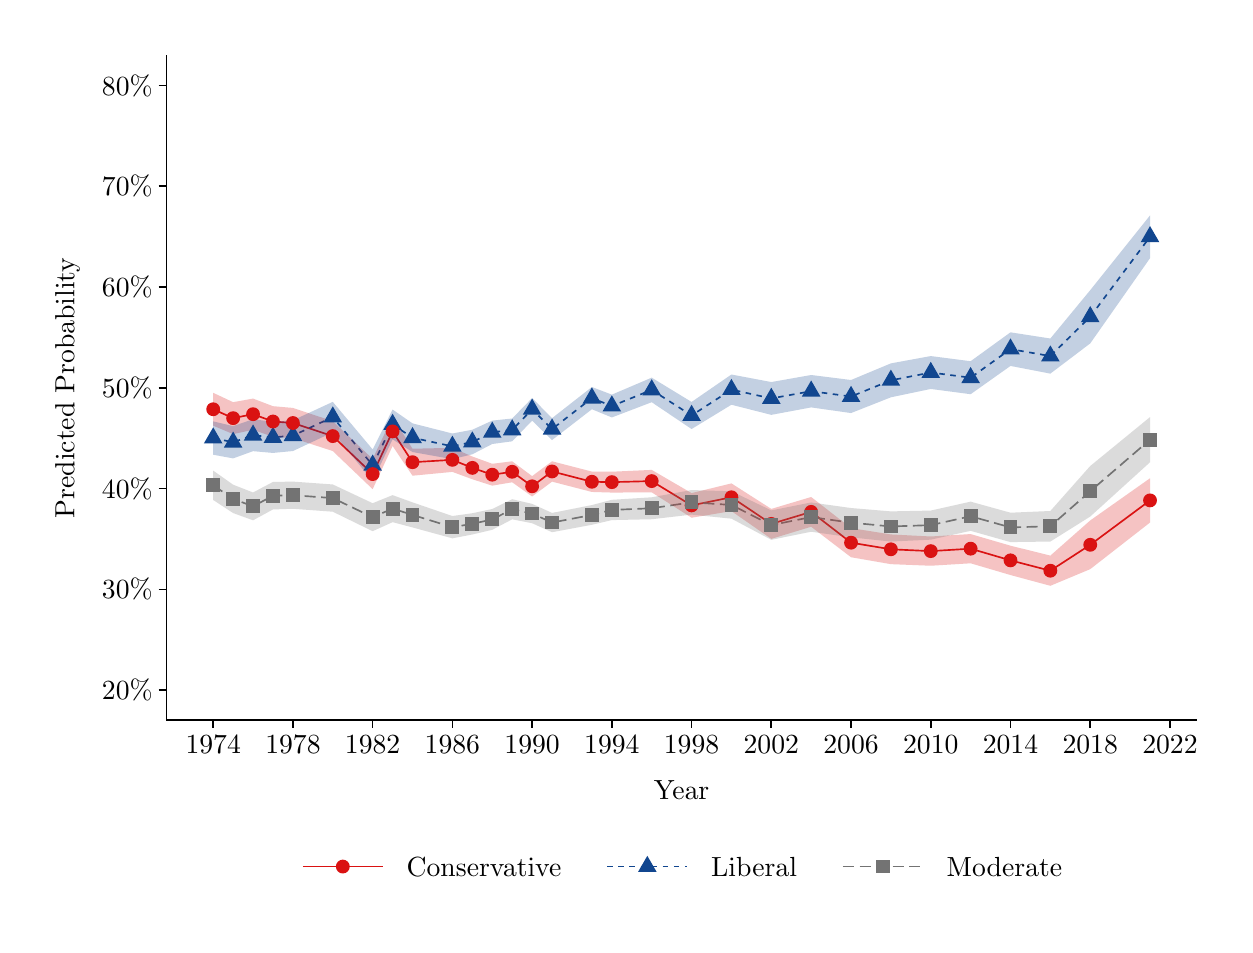
\begin{tikzpicture}[x=1pt,y=1pt]
\definecolor{fillColor}{RGB}{255,255,255}
\path[use as bounding box,fill=fillColor,fill opacity=0.00] (0,0) rectangle (432.48,324.36);
\begin{scope}
\path[clip] (  0.00,  0.00) rectangle (432.48,324.36);
\definecolor{fillColor}{RGB}{255,255,255}

\path[fill=fillColor] ( -0.00,  0.00) rectangle (432.48,324.36);
\end{scope}
\begin{scope}
\path[clip] ( 50.11, 74.07) rectangle (422.48,314.36);
\definecolor{fillColor}{RGB}{255,255,255}

\path[fill=fillColor] ( 50.11, 74.07) rectangle (422.48,314.36);
\definecolor{drawColor}{RGB}{218,18,18}

\path[draw=drawColor,line width= 0.6pt,line join=round] ( 67.04,186.47) --
	( 74.24,183.26) --
	( 81.44,184.69) --
	( 88.64,182.05) --
	( 95.85,181.50) --
	(110.25,176.77) --
	(124.66,163.05) --
	(131.86,178.47) --
	(139.06,167.34) --
	(153.47,168.19) --
	(160.67,165.29) --
	(167.87,162.82) --
	(175.07,163.88) --
	(182.28,158.63) --
	(189.48,164.00) --
	(203.88,160.27) --
	(211.09,160.14) --
	(225.49,160.51) --
	(239.90,151.73) --
	(254.30,154.67) --
	(268.71,145.05) --
	(283.11,149.39) --
	(297.52,138.26) --
	(311.92,135.87) --
	(326.33,135.21) --
	(340.73,136.09) --
	(355.14,131.87) --
	(369.54,128.13) --
	(383.95,137.49) --
	(405.56,153.54);
\definecolor{drawColor}{RGB}{17,70,143}

\path[draw=drawColor,line width= 0.6pt,dash pattern=on 2pt off 2pt ,line join=round] ( 67.04,176.07) --
	( 74.24,174.55) --
	( 81.44,177.10) --
	( 88.64,176.31) --
	( 95.85,176.93) --
	(110.25,183.65) --
	(124.66,166.24) --
	(131.86,180.98) --
	(139.06,176.19) --
	(153.47,173.07) --
	(160.67,174.64) --
	(167.87,178.15) --
	(175.07,179.01) --
	(182.28,186.45) --
	(189.48,179.29) --
	(203.88,190.50) --
	(211.09,187.63) --
	(225.49,193.46) --
	(239.90,184.22) --
	(254.30,193.57) --
	(268.71,190.38) --
	(283.11,193.00) --
	(297.52,191.07) --
	(311.92,196.92) --
	(326.33,199.75) --
	(340.73,197.87) --
	(355.14,208.20) --
	(369.54,205.69) --
	(383.95,219.89) --
	(405.56,248.79);
\definecolor{drawColor}{gray}{0.45}

\path[draw=drawColor,line width= 0.6pt,dash pattern=on 4pt off 2pt ,line join=round] ( 67.04,158.99) --
	( 74.24,154.08) --
	( 81.44,151.38) --
	( 88.64,155.24) --
	( 95.85,155.42) --
	(110.25,154.37) --
	(124.66,147.47) --
	(131.86,150.56) --
	(139.06,148.30) --
	(153.47,143.86) --
	(160.67,145.06) --
	(167.87,146.67) --
	(175.07,150.34) --
	(182.28,148.79) --
	(189.48,145.53) --
	(203.88,148.29) --
	(211.09,150.09) --
	(225.49,150.70) --
	(239.90,152.84) --
	(254.30,151.89) --
	(268.71,144.61) --
	(283.11,147.51) --
	(297.52,145.49) --
	(311.92,144.12) --
	(326.33,144.60) --
	(340.73,147.81) --
	(355.14,143.78) --
	(369.54,144.19) --
	(383.95,156.84) --
	(405.56,175.49);
\definecolor{fillColor}{RGB}{218,18,18}

\path[fill=fillColor,fill opacity=0.25] ( 67.04,192.41) --
	( 74.24,189.03) --
	( 81.44,190.33) --
	( 88.64,187.58) --
	( 95.85,186.95) --
	(110.25,182.17) --
	(124.66,168.52) --
	(131.86,183.73) --
	(139.06,172.21) --
	(153.47,172.53) --
	(160.67,169.40) --
	(167.87,166.77) --
	(175.07,167.66) --
	(182.28,162.31) --
	(189.48,167.67) --
	(203.88,163.95) --
	(211.09,163.90) --
	(225.49,164.56) --
	(239.90,156.17) --
	(254.30,159.68) --
	(268.71,150.46) --
	(283.11,154.77) --
	(297.52,143.52) --
	(311.92,141.24) --
	(326.33,140.50) --
	(340.73,141.37) --
	(355.14,137.17) --
	(369.54,133.58) --
	(383.95,146.29) --
	(405.56,161.54) --
	(405.56,145.55) --
	(383.95,128.70) --
	(369.54,122.68) --
	(355.14,126.57) --
	(340.73,130.81) --
	(326.33,129.93) --
	(311.92,130.50) --
	(297.52,133.00) --
	(283.11,144.01) --
	(268.71,139.64) --
	(254.30,149.66) --
	(239.90,147.28) --
	(225.49,156.45) --
	(211.09,156.37) --
	(203.88,156.59) --
	(189.48,160.32) --
	(182.28,154.95) --
	(175.07,160.09) --
	(167.87,158.87) --
	(160.67,161.18) --
	(153.47,163.84) --
	(139.06,162.46) --
	(131.86,173.20) --
	(124.66,157.59) --
	(110.25,171.37) --
	( 95.85,176.05) --
	( 88.64,176.52) --
	( 81.44,179.04) --
	( 74.24,177.50) --
	( 67.04,180.53) --
	cycle;

\path[] ( 67.04,192.41) --
	( 74.24,189.03) --
	( 81.44,190.33) --
	( 88.64,187.58) --
	( 95.85,186.95) --
	(110.25,182.17) --
	(124.66,168.52) --
	(131.86,183.73) --
	(139.06,172.21) --
	(153.47,172.53) --
	(160.67,169.40) --
	(167.87,166.77) --
	(175.07,167.66) --
	(182.28,162.31) --
	(189.48,167.67) --
	(203.88,163.95) --
	(211.09,163.90) --
	(225.49,164.56) --
	(239.90,156.17) --
	(254.30,159.68) --
	(268.71,150.46) --
	(283.11,154.77) --
	(297.52,143.52) --
	(311.92,141.24) --
	(326.33,140.50) --
	(340.73,141.37) --
	(355.14,137.17) --
	(369.54,133.58) --
	(383.95,146.29) --
	(405.56,161.54);

\path[] (405.56,145.55) --
	(383.95,128.70) --
	(369.54,122.68) --
	(355.14,126.57) --
	(340.73,130.81) --
	(326.33,129.93) --
	(311.92,130.50) --
	(297.52,133.00) --
	(283.11,144.01) --
	(268.71,139.64) --
	(254.30,149.66) --
	(239.90,147.28) --
	(225.49,156.45) --
	(211.09,156.37) --
	(203.88,156.59) --
	(189.48,160.32) --
	(182.28,154.95) --
	(175.07,160.09) --
	(167.87,158.87) --
	(160.67,161.18) --
	(153.47,163.84) --
	(139.06,162.46) --
	(131.86,173.20) --
	(124.66,157.59) --
	(110.25,171.37) --
	( 95.85,176.05) --
	( 88.64,176.52) --
	( 81.44,179.04) --
	( 74.24,177.50) --
	( 67.04,180.53);
\definecolor{fillColor}{RGB}{17,70,143}

\path[fill=fillColor,fill opacity=0.25] ( 67.04,182.09) --
	( 74.24,180.38) --
	( 81.44,182.87) --
	( 88.64,181.92) --
	( 95.85,182.48) --
	(110.25,189.14) --
	(124.66,171.95) --
	(131.86,186.36) --
	(139.06,181.37) --
	(153.47,177.71) --
	(160.67,179.07) --
	(167.87,182.37) --
	(175.07,183.13) --
	(182.28,190.53) --
	(189.48,183.25) --
	(203.88,194.51) --
	(211.09,191.75) --
	(225.49,197.89) --
	(239.90,189.11) --
	(254.30,199.03) --
	(268.71,196.30) --
	(283.11,198.85) --
	(297.52,197.04) --
	(311.92,203.05) --
	(326.33,205.69) --
	(340.73,203.83) --
	(355.14,214.27) --
	(369.54,212.03) --
	(383.95,229.50) --
	(405.56,256.52) --
	(405.56,241.07) --
	(383.95,210.27) --
	(369.54,199.35) --
	(355.14,202.13) --
	(340.73,191.91) --
	(326.33,193.81) --
	(311.92,190.79) --
	(297.52,185.10) --
	(283.11,187.14) --
	(268.71,184.45) --
	(254.30,188.11) --
	(239.90,179.33) --
	(225.49,189.02) --
	(211.09,183.51) --
	(203.88,186.48) --
	(189.48,175.34) --
	(182.28,182.36) --
	(175.07,174.89) --
	(167.87,173.92) --
	(160.67,170.20) --
	(153.47,168.44) --
	(139.06,171.01) --
	(131.86,175.60) --
	(124.66,160.54) --
	(110.25,178.15) --
	( 95.85,171.38) --
	( 88.64,170.69) --
	( 81.44,171.33) --
	( 74.24,168.72) --
	( 67.04,170.04) --
	cycle;

\path[] ( 67.04,182.09) --
	( 74.24,180.38) --
	( 81.44,182.87) --
	( 88.64,181.92) --
	( 95.85,182.48) --
	(110.25,189.14) --
	(124.66,171.95) --
	(131.86,186.36) --
	(139.06,181.37) --
	(153.47,177.71) --
	(160.67,179.07) --
	(167.87,182.37) --
	(175.07,183.13) --
	(182.28,190.53) --
	(189.48,183.25) --
	(203.88,194.51) --
	(211.09,191.75) --
	(225.49,197.89) --
	(239.90,189.11) --
	(254.30,199.03) --
	(268.71,196.30) --
	(283.11,198.85) --
	(297.52,197.04) --
	(311.92,203.05) --
	(326.33,205.69) --
	(340.73,203.83) --
	(355.14,214.27) --
	(369.54,212.03) --
	(383.95,229.50) --
	(405.56,256.52);

\path[] (405.56,241.07) --
	(383.95,210.27) --
	(369.54,199.35) --
	(355.14,202.13) --
	(340.73,191.91) --
	(326.33,193.81) --
	(311.92,190.79) --
	(297.52,185.10) --
	(283.11,187.14) --
	(268.71,184.45) --
	(254.30,188.11) --
	(239.90,179.33) --
	(225.49,189.02) --
	(211.09,183.51) --
	(203.88,186.48) --
	(189.48,175.34) --
	(182.28,182.36) --
	(175.07,174.89) --
	(167.87,173.92) --
	(160.67,170.20) --
	(153.47,168.44) --
	(139.06,171.01) --
	(131.86,175.60) --
	(124.66,160.54) --
	(110.25,178.15) --
	( 95.85,171.38) --
	( 88.64,170.69) --
	( 81.44,171.33) --
	( 74.24,168.72) --
	( 67.04,170.04);
\definecolor{fillColor}{RGB}{115,115,115}

\path[fill=fillColor,fill opacity=0.25] ( 67.04,164.30) --
	( 74.24,159.21) --
	( 81.44,156.40) --
	( 88.64,160.20) --
	( 95.85,160.33) --
	(110.25,159.30) --
	(124.66,152.52) --
	(131.86,155.44) --
	(139.06,152.83) --
	(153.47,147.89) --
	(160.67,148.90) --
	(167.87,150.43) --
	(175.07,153.97) --
	(182.28,152.29) --
	(189.48,149.01) --
	(203.88,151.85) --
	(211.09,153.75) --
	(225.49,154.66) --
	(239.90,157.28) --
	(254.30,156.84) --
	(268.71,149.93) --
	(283.11,152.79) --
	(297.52,150.78) --
	(311.92,149.57) --
	(326.33,149.86) --
	(340.73,153.09) --
	(355.14,149.09) --
	(369.54,149.71) --
	(383.95,165.97) --
	(405.56,183.65) --
	(405.56,167.33) --
	(383.95,147.70) --
	(369.54,138.67) --
	(355.14,138.47) --
	(340.73,142.54) --
	(326.33,139.35) --
	(311.92,138.67) --
	(297.52,140.19) --
	(283.11,142.22) --
	(268.71,139.29) --
	(254.30,146.94) --
	(239.90,148.40) --
	(225.49,146.73) --
	(211.09,146.42) --
	(203.88,144.73) --
	(189.48,142.04) --
	(182.28,145.29) --
	(175.07,146.70) --
	(167.87,142.91) --
	(160.67,141.22) --
	(153.47,139.83) --
	(139.06,143.77) --
	(131.86,145.68) --
	(124.66,142.41) --
	(110.25,149.45) --
	( 95.85,150.51) --
	( 88.64,150.27) --
	( 81.44,146.35) --
	( 74.24,148.96) --
	( 67.04,153.69) --
	cycle;

\path[] ( 67.04,164.30) --
	( 74.24,159.21) --
	( 81.44,156.40) --
	( 88.64,160.20) --
	( 95.85,160.33) --
	(110.25,159.30) --
	(124.66,152.52) --
	(131.86,155.44) --
	(139.06,152.83) --
	(153.47,147.89) --
	(160.67,148.90) --
	(167.87,150.43) --
	(175.07,153.97) --
	(182.28,152.29) --
	(189.48,149.01) --
	(203.88,151.85) --
	(211.09,153.75) --
	(225.49,154.66) --
	(239.90,157.28) --
	(254.30,156.84) --
	(268.71,149.93) --
	(283.11,152.79) --
	(297.52,150.78) --
	(311.92,149.57) --
	(326.33,149.86) --
	(340.73,153.09) --
	(355.14,149.09) --
	(369.54,149.71) --
	(383.95,165.97) --
	(405.56,183.65);

\path[] (405.56,167.33) --
	(383.95,147.70) --
	(369.54,138.67) --
	(355.14,138.47) --
	(340.73,142.54) --
	(326.33,139.35) --
	(311.92,138.67) --
	(297.52,140.19) --
	(283.11,142.22) --
	(268.71,139.29) --
	(254.30,146.94) --
	(239.90,148.40) --
	(225.49,146.73) --
	(211.09,146.42) --
	(203.88,144.73) --
	(189.48,142.04) --
	(182.28,145.29) --
	(175.07,146.70) --
	(167.87,142.91) --
	(160.67,141.22) --
	(153.47,139.83) --
	(139.06,143.77) --
	(131.86,145.68) --
	(124.66,142.41) --
	(110.25,149.45) --
	( 95.85,150.51) --
	( 88.64,150.27) --
	( 81.44,146.35) --
	( 74.24,148.96) --
	( 67.04,153.69);
\definecolor{fillColor}{RGB}{17,70,143}

\path[fill=fillColor] ( 67.04,179.95) --
	( 70.40,174.12) --
	( 63.67,174.12) --
	cycle;

\path[fill=fillColor] ( 74.24,178.43) --
	( 77.60,172.60) --
	( 70.87,172.60) --
	cycle;

\path[fill=fillColor] ( 81.44,180.99) --
	( 84.80,175.16) --
	( 78.08,175.16) --
	cycle;

\path[fill=fillColor] ( 88.64,180.19) --
	( 92.01,174.36) --
	( 85.28,174.36) --
	cycle;

\path[fill=fillColor] ( 95.85,180.81) --
	( 99.21,174.99) --
	( 92.48,174.99) --
	cycle;

\path[fill=fillColor] (110.25,187.53) --
	(113.62,181.70) --
	(106.89,181.70) --
	cycle;

\path[fill=fillColor] (124.66,170.13) --
	(128.02,164.30) --
	(121.29,164.30) --
	cycle;

\path[fill=fillColor] (131.86,184.87) --
	(135.22,179.04) --
	(128.50,179.04) --
	cycle;

\path[fill=fillColor] (139.06,180.07) --
	(142.43,174.25) --
	(135.70,174.25) --
	cycle;

\path[fill=fillColor] (153.47,176.96) --
	(156.83,171.13) --
	(150.10,171.13) --
	cycle;

\path[fill=fillColor] (160.67,178.52) --
	(164.03,172.69) --
	(157.31,172.69) --
	cycle;

\path[fill=fillColor] (167.87,182.03) --
	(171.24,176.20) --
	(164.51,176.20) --
	cycle;

\path[fill=fillColor] (175.07,182.89) --
	(178.44,177.07) --
	(171.71,177.07) --
	cycle;

\path[fill=fillColor] (182.28,190.33) --
	(185.64,184.51) --
	(178.91,184.51) --
	cycle;

\path[fill=fillColor] (189.48,183.18) --
	(192.84,177.35) --
	(186.12,177.35) --
	cycle;

\path[fill=fillColor] (203.88,194.38) --
	(207.25,188.55) --
	(200.52,188.55) --
	cycle;

\path[fill=fillColor] (211.09,191.51) --
	(214.45,185.68) --
	(207.72,185.68) --
	cycle;

\path[fill=fillColor] (225.49,197.34) --
	(228.86,191.51) --
	(222.13,191.51) --
	cycle;

\path[fill=fillColor] (239.90,188.11) --
	(243.26,182.28) --
	(236.53,182.28) --
	cycle;

\path[fill=fillColor] (254.30,197.45) --
	(257.67,191.63) --
	(250.94,191.63) --
	cycle;

\path[fill=fillColor] (268.71,194.26) --
	(272.07,188.44) --
	(265.34,188.44) --
	cycle;

\path[fill=fillColor] (283.11,196.88) --
	(286.48,191.05) --
	(279.75,191.05) --
	cycle;

\path[fill=fillColor] (297.52,194.96) --
	(300.88,189.13) --
	(294.15,189.13) --
	cycle;

\path[fill=fillColor] (311.92,200.81) --
	(315.29,194.98) --
	(308.56,194.98) --
	cycle;

\path[fill=fillColor] (326.33,203.63) --
	(329.69,197.81) --
	(322.96,197.81) --
	cycle;

\path[fill=fillColor] (340.73,201.75) --
	(344.10,195.93) --
	(337.37,195.93) --
	cycle;

\path[fill=fillColor] (355.14,212.09) --
	(358.50,206.26) --
	(351.77,206.26) --
	cycle;

\path[fill=fillColor] (369.54,209.57) --
	(372.91,203.75) --
	(366.18,203.75) --
	cycle;

\path[fill=fillColor] (383.95,223.77) --
	(387.31,217.94) --
	(380.58,217.94) --
	cycle;

\path[fill=fillColor] (405.56,252.68) --
	(408.92,246.85) --
	(402.19,246.85) --
	cycle;
\definecolor{fillColor}{RGB}{218,18,18}

\path[fill=fillColor] ( 67.04,186.47) circle (  2.50);

\path[fill=fillColor] ( 74.24,183.26) circle (  2.50);

\path[fill=fillColor] ( 81.44,184.69) circle (  2.50);

\path[fill=fillColor] ( 88.64,182.05) circle (  2.50);

\path[fill=fillColor] ( 95.85,181.50) circle (  2.50);

\path[fill=fillColor] (110.25,176.77) circle (  2.50);

\path[fill=fillColor] (124.66,163.05) circle (  2.50);

\path[fill=fillColor] (131.86,178.47) circle (  2.50);

\path[fill=fillColor] (139.06,167.34) circle (  2.50);

\path[fill=fillColor] (153.47,168.19) circle (  2.50);

\path[fill=fillColor] (160.67,165.29) circle (  2.50);

\path[fill=fillColor] (167.87,162.82) circle (  2.50);

\path[fill=fillColor] (175.07,163.88) circle (  2.50);

\path[fill=fillColor] (182.28,158.63) circle (  2.50);

\path[fill=fillColor] (189.48,164.00) circle (  2.50);

\path[fill=fillColor] (203.88,160.27) circle (  2.50);

\path[fill=fillColor] (211.09,160.14) circle (  2.50);

\path[fill=fillColor] (225.49,160.51) circle (  2.50);

\path[fill=fillColor] (239.90,151.73) circle (  2.50);

\path[fill=fillColor] (254.30,154.67) circle (  2.50);

\path[fill=fillColor] (268.71,145.05) circle (  2.50);

\path[fill=fillColor] (283.11,149.39) circle (  2.50);

\path[fill=fillColor] (297.52,138.26) circle (  2.50);

\path[fill=fillColor] (311.92,135.87) circle (  2.50);

\path[fill=fillColor] (326.33,135.21) circle (  2.50);

\path[fill=fillColor] (340.73,136.09) circle (  2.50);

\path[fill=fillColor] (355.14,131.87) circle (  2.50);

\path[fill=fillColor] (369.54,128.13) circle (  2.50);

\path[fill=fillColor] (383.95,137.49) circle (  2.50);

\path[fill=fillColor] (405.56,153.54) circle (  2.50);
\definecolor{fillColor}{gray}{0.45}

\path[fill=fillColor] ( 64.54,156.50) --
	( 69.53,156.50) --
	( 69.53,161.49) --
	( 64.54,161.49) --
	cycle;

\path[fill=fillColor] ( 71.74,151.58) --
	( 76.74,151.58) --
	( 76.74,156.58) --
	( 71.74,156.58) --
	cycle;

\path[fill=fillColor] ( 78.94,148.88) --
	( 83.94,148.88) --
	( 83.94,153.88) --
	( 78.94,153.88) --
	cycle;

\path[fill=fillColor] ( 86.15,152.74) --
	( 91.14,152.74) --
	( 91.14,157.73) --
	( 86.15,157.73) --
	cycle;

\path[fill=fillColor] ( 93.35,152.92) --
	( 98.34,152.92) --
	( 98.34,157.92) --
	( 93.35,157.92) --
	cycle;

\path[fill=fillColor] (107.75,151.88) --
	(112.75,151.88) --
	(112.75,156.87) --
	(107.75,156.87) --
	cycle;

\path[fill=fillColor] (122.16,144.97) --
	(127.15,144.97) --
	(127.15,149.97) --
	(122.16,149.97) --
	cycle;

\path[fill=fillColor] (129.36,148.06) --
	(134.36,148.06) --
	(134.36,153.06) --
	(129.36,153.06) --
	cycle;

\path[fill=fillColor] (136.56,145.81) --
	(141.56,145.81) --
	(141.56,150.80) --
	(136.56,150.80) --
	cycle;

\path[fill=fillColor] (150.97,141.36) --
	(155.96,141.36) --
	(155.96,146.36) --
	(150.97,146.36) --
	cycle;

\path[fill=fillColor] (158.17,142.56) --
	(163.17,142.56) --
	(163.17,147.56) --
	(158.17,147.56) --
	cycle;

\path[fill=fillColor] (165.37,144.17) --
	(170.37,144.17) --
	(170.37,149.17) --
	(165.37,149.17) --
	cycle;

\path[fill=fillColor] (172.58,147.84) --
	(177.57,147.84) --
	(177.57,152.84) --
	(172.58,152.84) --
	cycle;

\path[fill=fillColor] (179.78,146.29) --
	(184.77,146.29) --
	(184.77,151.29) --
	(179.78,151.29) --
	cycle;

\path[fill=fillColor] (186.98,143.03) --
	(191.98,143.03) --
	(191.98,148.03) --
	(186.98,148.03) --
	cycle;

\path[fill=fillColor] (201.39,145.79) --
	(206.38,145.79) --
	(206.38,150.79) --
	(201.39,150.79) --
	cycle;

\path[fill=fillColor] (208.59,147.59) --
	(213.58,147.59) --
	(213.58,152.58) --
	(208.59,152.58) --
	cycle;

\path[fill=fillColor] (222.99,148.20) --
	(227.99,148.20) --
	(227.99,153.20) --
	(222.99,153.20) --
	cycle;

\path[fill=fillColor] (237.40,150.34) --
	(242.39,150.34) --
	(242.39,155.34) --
	(237.40,155.34) --
	cycle;

\path[fill=fillColor] (251.80,149.39) --
	(256.80,149.39) --
	(256.80,154.39) --
	(251.80,154.39) --
	cycle;

\path[fill=fillColor] (266.21,142.11) --
	(271.21,142.11) --
	(271.21,147.11) --
	(266.21,147.11) --
	cycle;

\path[fill=fillColor] (280.61,145.01) --
	(285.61,145.01) --
	(285.61,150.00) --
	(280.61,150.00) --
	cycle;

\path[fill=fillColor] (295.02,142.99) --
	(300.02,142.99) --
	(300.02,147.98) --
	(295.02,147.98) --
	cycle;

\path[fill=fillColor] (309.43,141.62) --
	(314.42,141.62) --
	(314.42,146.62) --
	(309.43,146.62) --
	cycle;

\path[fill=fillColor] (323.83,142.11) --
	(328.83,142.11) --
	(328.83,147.10) --
	(323.83,147.10) --
	cycle;

\path[fill=fillColor] (338.24,145.32) --
	(343.23,145.32) --
	(343.23,150.31) --
	(338.24,150.31) --
	cycle;

\path[fill=fillColor] (352.64,141.28) --
	(357.64,141.28) --
	(357.64,146.28) --
	(352.64,146.28) --
	cycle;

\path[fill=fillColor] (367.05,141.69) --
	(372.04,141.69) --
	(372.04,146.69) --
	(367.05,146.69) --
	cycle;

\path[fill=fillColor] (381.45,154.34) --
	(386.45,154.34) --
	(386.45,159.34) --
	(381.45,159.34) --
	cycle;

\path[fill=fillColor] (403.06,172.99) --
	(408.05,172.99) --
	(408.05,177.99) --
	(403.06,177.99) --
	cycle;
\end{scope}
\begin{scope}
\path[clip] (  0.00,  0.00) rectangle (432.48,324.36);
\definecolor{drawColor}{RGB}{0,0,0}

\path[draw=drawColor,line width= 0.6pt,line join=round] ( 50.11, 74.07) --
	( 50.11,314.36);
\end{scope}
\begin{scope}
\path[clip] (  0.00,  0.00) rectangle (432.48,324.36);
\definecolor{drawColor}{RGB}{0,0,0}

\node[text=drawColor,anchor=base east,inner sep=0pt, outer sep=0pt, scale=  1.00] at ( 45.16, 81.55) {20{\%}};

\node[text=drawColor,anchor=base east,inner sep=0pt, outer sep=0pt, scale=  1.00] at ( 45.16,117.95) {30{\%}};

\node[text=drawColor,anchor=base east,inner sep=0pt, outer sep=0pt, scale=  1.00] at ( 45.16,154.36) {40{\%}};

\node[text=drawColor,anchor=base east,inner sep=0pt, outer sep=0pt, scale=  1.00] at ( 45.16,190.77) {50{\%}};

\node[text=drawColor,anchor=base east,inner sep=0pt, outer sep=0pt, scale=  1.00] at ( 45.16,227.18) {60{\%}};

\node[text=drawColor,anchor=base east,inner sep=0pt, outer sep=0pt, scale=  1.00] at ( 45.16,263.59) {70{\%}};

\node[text=drawColor,anchor=base east,inner sep=0pt, outer sep=0pt, scale=  1.00] at ( 45.16,300.00) {80{\%}};
\end{scope}
\begin{scope}
\path[clip] (  0.00,  0.00) rectangle (432.48,324.36);
\definecolor{drawColor}{RGB}{0,0,0}

\path[draw=drawColor,line width= 0.6pt,line join=round] ( 47.36, 84.99) --
	( 50.11, 84.99);

\path[draw=drawColor,line width= 0.6pt,line join=round] ( 47.36,121.40) --
	( 50.11,121.40);

\path[draw=drawColor,line width= 0.6pt,line join=round] ( 47.36,157.81) --
	( 50.11,157.81);

\path[draw=drawColor,line width= 0.6pt,line join=round] ( 47.36,194.21) --
	( 50.11,194.21);

\path[draw=drawColor,line width= 0.6pt,line join=round] ( 47.36,230.62) --
	( 50.11,230.62);

\path[draw=drawColor,line width= 0.6pt,line join=round] ( 47.36,267.03) --
	( 50.11,267.03);

\path[draw=drawColor,line width= 0.6pt,line join=round] ( 47.36,303.44) --
	( 50.11,303.44);
\end{scope}
\begin{scope}
\path[clip] (  0.00,  0.00) rectangle (432.48,324.36);
\definecolor{drawColor}{RGB}{0,0,0}

\path[draw=drawColor,line width= 0.6pt,line join=round] ( 50.11, 74.07) --
	(422.48, 74.07);
\end{scope}
\begin{scope}
\path[clip] (  0.00,  0.00) rectangle (432.48,324.36);
\definecolor{drawColor}{RGB}{0,0,0}

\path[draw=drawColor,line width= 0.6pt,line join=round] ( 67.04, 71.32) --
	( 67.04, 74.07);

\path[draw=drawColor,line width= 0.6pt,line join=round] ( 95.85, 71.32) --
	( 95.85, 74.07);

\path[draw=drawColor,line width= 0.6pt,line join=round] (124.66, 71.32) --
	(124.66, 74.07);

\path[draw=drawColor,line width= 0.6pt,line join=round] (153.47, 71.32) --
	(153.47, 74.07);

\path[draw=drawColor,line width= 0.6pt,line join=round] (182.28, 71.32) --
	(182.28, 74.07);

\path[draw=drawColor,line width= 0.6pt,line join=round] (211.09, 71.32) --
	(211.09, 74.07);

\path[draw=drawColor,line width= 0.6pt,line join=round] (239.90, 71.32) --
	(239.90, 74.07);

\path[draw=drawColor,line width= 0.6pt,line join=round] (268.71, 71.32) --
	(268.71, 74.07);

\path[draw=drawColor,line width= 0.6pt,line join=round] (297.52, 71.32) --
	(297.52, 74.07);

\path[draw=drawColor,line width= 0.6pt,line join=round] (326.33, 71.32) --
	(326.33, 74.07);

\path[draw=drawColor,line width= 0.6pt,line join=round] (355.14, 71.32) --
	(355.14, 74.07);

\path[draw=drawColor,line width= 0.6pt,line join=round] (383.95, 71.32) --
	(383.95, 74.07);

\path[draw=drawColor,line width= 0.6pt,line join=round] (412.76, 71.32) --
	(412.76, 74.07);
\end{scope}
\begin{scope}
\path[clip] (  0.00,  0.00) rectangle (432.48,324.36);
\definecolor{drawColor}{RGB}{0,0,0}

\node[text=drawColor,anchor=base,inner sep=0pt, outer sep=0pt, scale=  1.00] at ( 67.04, 62.23) {1974};

\node[text=drawColor,anchor=base,inner sep=0pt, outer sep=0pt, scale=  1.00] at ( 95.85, 62.23) {1978};

\node[text=drawColor,anchor=base,inner sep=0pt, outer sep=0pt, scale=  1.00] at (124.66, 62.23) {1982};

\node[text=drawColor,anchor=base,inner sep=0pt, outer sep=0pt, scale=  1.00] at (153.47, 62.23) {1986};

\node[text=drawColor,anchor=base,inner sep=0pt, outer sep=0pt, scale=  1.00] at (182.28, 62.23) {1990};

\node[text=drawColor,anchor=base,inner sep=0pt, outer sep=0pt, scale=  1.00] at (211.09, 62.23) {1994};

\node[text=drawColor,anchor=base,inner sep=0pt, outer sep=0pt, scale=  1.00] at (239.90, 62.23) {1998};

\node[text=drawColor,anchor=base,inner sep=0pt, outer sep=0pt, scale=  1.00] at (268.71, 62.23) {2002};

\node[text=drawColor,anchor=base,inner sep=0pt, outer sep=0pt, scale=  1.00] at (297.52, 62.23) {2006};

\node[text=drawColor,anchor=base,inner sep=0pt, outer sep=0pt, scale=  1.00] at (326.33, 62.23) {2010};

\node[text=drawColor,anchor=base,inner sep=0pt, outer sep=0pt, scale=  1.00] at (355.14, 62.23) {2014};

\node[text=drawColor,anchor=base,inner sep=0pt, outer sep=0pt, scale=  1.00] at (383.95, 62.23) {2018};

\node[text=drawColor,anchor=base,inner sep=0pt, outer sep=0pt, scale=  1.00] at (412.76, 62.23) {2022};
\end{scope}
\begin{scope}
\path[clip] (  0.00,  0.00) rectangle (432.48,324.36);
\definecolor{drawColor}{RGB}{0,0,0}

\node[text=drawColor,anchor=base,inner sep=0pt, outer sep=0pt, scale=  1.00] at (236.30, 45.40) {Year};
\end{scope}
\begin{scope}
\path[clip] (  0.00,  0.00) rectangle (432.48,324.36);
\definecolor{drawColor}{RGB}{0,0,0}

\node[text=drawColor,rotate= 90.00,anchor=base,inner sep=0pt, outer sep=0pt, scale=  1.00] at ( 16.89,194.21) {Predicted Probability};
\end{scope}
\begin{scope}
\path[clip] (  0.00,  0.00) rectangle (432.48,324.36);

\path[] ( 86.80, 10.00) rectangle (385.79, 32.45);
\end{scope}
\begin{scope}
\path[clip] (  0.00,  0.00) rectangle (432.48,324.36);

\path[] ( 95.80, 14.00) rectangle (131.94, 28.45);
\end{scope}
\begin{scope}
\path[clip] (  0.00,  0.00) rectangle (432.48,324.36);
\definecolor{drawColor}{RGB}{218,18,18}

\path[draw=drawColor,line width= 0.6pt,line join=round] ( 99.42, 21.23) -- (128.33, 21.23);
\end{scope}
\begin{scope}
\path[clip] (  0.00,  0.00) rectangle (432.48,324.36);
\definecolor{fillColor}{RGB}{218,18,18}

\path[fill=fillColor] (113.87, 21.23) circle (  2.50);
\end{scope}
\begin{scope}
\path[clip] (  0.00,  0.00) rectangle (432.48,324.36);

\path[] (205.84, 14.00) rectangle (241.98, 28.45);
\end{scope}
\begin{scope}
\path[clip] (  0.00,  0.00) rectangle (432.48,324.36);
\definecolor{drawColor}{RGB}{17,70,143}

\path[draw=drawColor,line width= 0.6pt,dash pattern=on 2pt off 2pt ,line join=round] (209.46, 21.23) -- (238.36, 21.23);
\end{scope}
\begin{scope}
\path[clip] (  0.00,  0.00) rectangle (432.48,324.36);
\definecolor{fillColor}{RGB}{17,70,143}

\path[fill=fillColor] (223.91, 25.11) --
	(227.27, 19.28) --
	(220.55, 19.28) --
	cycle;
\end{scope}
\begin{scope}
\path[clip] (  0.00,  0.00) rectangle (432.48,324.36);

\path[] (290.97, 14.00) rectangle (327.10, 28.45);
\end{scope}
\begin{scope}
\path[clip] (  0.00,  0.00) rectangle (432.48,324.36);
\definecolor{drawColor}{gray}{0.45}

\path[draw=drawColor,line width= 0.6pt,dash pattern=on 4pt off 2pt ,line join=round] (294.58, 21.23) -- (323.49, 21.23);
\end{scope}
\begin{scope}
\path[clip] (  0.00,  0.00) rectangle (432.48,324.36);
\definecolor{fillColor}{gray}{0.45}

\path[fill=fillColor] (306.54, 18.73) --
	(311.53, 18.73) --
	(311.53, 23.72) --
	(306.54, 23.72) --
	cycle;
\end{scope}
\begin{scope}
\path[clip] (  0.00,  0.00) rectangle (432.48,324.36);
\definecolor{drawColor}{RGB}{0,0,0}

\node[text=drawColor,anchor=base west,inner sep=0pt, outer sep=0pt, scale=  1.00] at (136.94, 17.78) {Conservative};
\end{scope}
\begin{scope}
\path[clip] (  0.00,  0.00) rectangle (432.48,324.36);
\definecolor{drawColor}{RGB}{0,0,0}

\node[text=drawColor,anchor=base west,inner sep=0pt, outer sep=0pt, scale=  1.00] at (246.98, 17.78) {Liberal};
\end{scope}
\begin{scope}
\path[clip] (  0.00,  0.00) rectangle (432.48,324.36);
\definecolor{drawColor}{RGB}{0,0,0}

\node[text=drawColor,anchor=base west,inner sep=0pt, outer sep=0pt, scale=  1.00] at (332.10, 17.78) {Moderate};
\end{scope}
\end{tikzpicture}
